\chapter{Herramientas Empleadas}\label{ch:herramientas}

En este capítulo se explican las herramientas, librerias y APIs que se han utilizado en el desarrollo de AdaptaMaterialEscolar 2.0. En la sección~\ref{sec:tailwind} se explica el framework Tailwind CSS. En la sección \ref{sec:Slate} se expone el framework Slate. En la sección \ref{sec:React} se presenta la libreria React. Y en la sección \ref{sec:MaterialUI} se explica qué es libería Material UI.

\section{Tailwind CSS}\label{sec:tailwind}
A continuación se explica que es Tailwind CSS, porque hemos decidido utilizarlo y que algunas de las ventajas que ofrece. Además se muestran y explican algunos ejemplos de uso básicos.

Tailwind CSS\footnote{\url{https://tailwindcss.com/}} es un framework CSS que permite aplicar estilos predefinidos directamente en el HTML sin tener que crear y manejar archivos CSS propios para conseguir un estilo concreto. Hemos decidido utilizar este framework porque facilita la labor de dar estilo al HTML de la página, debido a que no tenemos que pensar en que clases o identificadores dar a los elementos HTML y, por lo general, tampoco necesitamos gestionar un archivo CSS por cada página o componente de React. Otra de las razones por las que hemos escogido este framework frente a otros muy parecidos, como Bootstrap\footnote{\url{https://getbootstrap.com/}}, es la facilidad que ofrece para personalizarlo y adaptarlo a nuestras necesidades. En el caso de Bootstrap, necesitas utilizar SASS o crear tus propios archivos CSS para poder mantener un esquema de colores, mientras que en Tailwind CSS modificando un archivo de configuración puedes añadir colores, cambiar el tipo de fuente, el tamaño de letra, etc. Otras ventajas que ofrece son:
\begin{itemize}
    \item \textbf{Rendimiento}: Tailwind elimina automáticamente todo el CSS que no se utilice a la hora de desplegar en producción la apliación, consiguiendo que el paquete de CSS que se envía al cliente sea lo más pequeño posible.
    \item \textbf{Diseño responsive}: Permite aplicar distintos estilos dependiendo del tamaño de la ventana sin necesidad de pelearse con media queries\footnote{\url{https://developer.mozilla.org/en-US/docs/Web/CSS/Media_Queries/Using_media_queries}} de CSS.
    \item \textbf{Reutilización}: Tailwind permite reutilizar conjuntos de utilidades que se repitan mucho definiendo una clase CSS propia que los aplique todos. Aun así, nosotros no utilizaremos, principalmente, el método que ofrece Tailwind para reutilizar estilos, ya que podemos conseguir el mismo resultado creando un componente de React, con la ventaja de poder añadir lógica de JavaScript.
\end{itemize}

% TODO: Añadir ejemplos de uso

\section{Slate}\label{sec:Slate}
Slate\footnote{\url{https://docs.slatejs.org/}} es un framework de JavaScript de código abierto que se utiliza para construir editores de texto "What You See Is What You Get" (WYSIWYG) personalizados. A diferencia de las bibliotecas de edición de texto tradicionales, Slate utiliza una estructura de árbol de datos para representar el contenido del editor y proporciona una API para manipular ese contenido.
\\
Las principales características de Slate incluyen:
\begin{itemize}
    \item \textbf{Personalización}: La biblioteca permite a los desarrolladores personalizar el editor de texto según sus necesidades, lo que significa que pueden definir sus propios tipos de nodos y componentes de renderizado.
    \item \textbf{Flexibilidad}: Al ser una biblioteca de JavaScript, SlateJS es altamente flexible y puede integrarse fácilmente con otras bibliotecas y marcos como React.
    \item \textbf{Rendimiento}: La estructura de árbol de datos utilizada por SlateJS permite que la biblioteca realice actualizaciones eficientes del DOM, lo que resulta en un editor de texto rápido y fluido.
    \item \textbf{Soporte de complementos}: Los complementos de SlateJS son módulos que proporcionan una funcionalidad adicional al editor de texto. Estos complementos pueden personalizarse y utilizarse según las necesidades del desarrollador.
    \item \textbf{Compatibilidad multiplataforma}: SlateJS es compatible con una amplia gama de navegadores y plataformas. 
\end{itemize}
Es utilizado por variedad de aplicaciones web como, por ejemplo:
\begin{itemize}
    \item \textbf{Discord}: Utiliza Slate para sus canales de comunicación para colaborar y compartir
    \item \textbf{Eraser}: Es una aplicación web de borrador de fondos que utiliza Slate para permitir a los usuarios escribir y editar el texto en su sitio web.
    \item \textbf{GitBook}: Es una plataforma de creación y publicación de libros electrónicos que utiliza Slate como editor de texto para que los autores puedan escribir y editar sus libros
    
\end{itemize}
Por todo lo mencionado, hemos considerado que Slate es ideal para este proyecto que busca construir un editor de texto de alta calidad que permite realizar diversos tipos de adaptación curricular.

\section{React}\label{sec:React}
React es una librería de JavaScript que se utiliza para crear interfaces de usuario interactivas y dinámicas en aplicaciones web. Fue desarrollada por Facebook y es una de las herramientas más populares para construir aplicaciones web modernas.

React utiliza un enfoque basado en componentes para construir interfaces de usuario, lo que significa que cada parte de la interfaz de usuario se representa como un componente. Dichos componentes son reutilizables y están diseñados para ser simples, fáciles de mantener y declarativos, es decir, describe qué se quiere hacer y no cómo hacerlo. Otras ventajas que ofrece son:

\begin{itemize}
    \item \textbf{Mayor eficiencia}: React utiliza un enfoque llamado "reconciliación virtual" para actualizar la interfaz de usuario de manera eficiente y minimizar el impacto en el rendimiento. Este enfoque se basa en la comparación de los estados previos y actuales de los componentes, permitiendo actualizar solo las partes necesarias de la interfaz.
    \item \textbf{Facilidad de mantenimiento}: Como se ha mencionado anteriormente los componentes de React son simples y declarativos, lo que hace que sea más fácil mantener y actualizar una aplicación web construida con React.
   \item \textbf{Biblioteca de componentes}: React tiene una gran biblioteca de componentes disponibles para su uso, lo que permite a los desarrolladores construir aplicaciones web complejas con facilidad.
\end{itemize}

Para representar las interfaces de usuario en React se utiliza una extensión de sintaxis llamada JSX que permite escribir HTML en JavaScript, lo que hace que el código sea más legible y fácil de entender. En JSX, los elementos de la interfaz de usuario se definen como etiquetas HTML dentro del código JavaScript. En la Figura \ref{JSX} se muestra un ejemplo de un componente usando JSX y en la Figura \ref{SJSX} se encuentra la misma funcionalidad pero sin JSX.

Hemos empleado esta librería para implementar las interfaces de usuario de la aplicación.
  \begin{figure}[ht!]
   
    \begin{subfigure}{\textwidth}
      \centering
      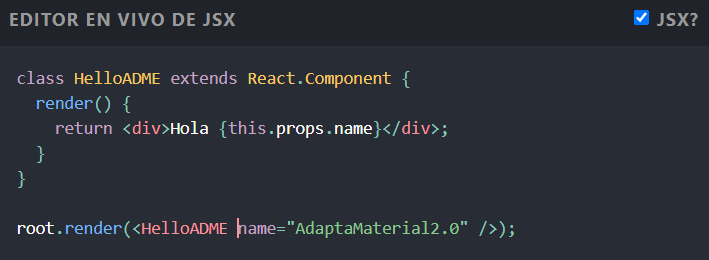
\includegraphics[width=0.6\textwidth]{Herraientas_Empleadas/ReactJSX.PNG}
      \caption{Componente con JSX.}
      \label{JSX}
    \end{subfigure}
  
    \begin{subfigure}{\textwidth}
      \centering
      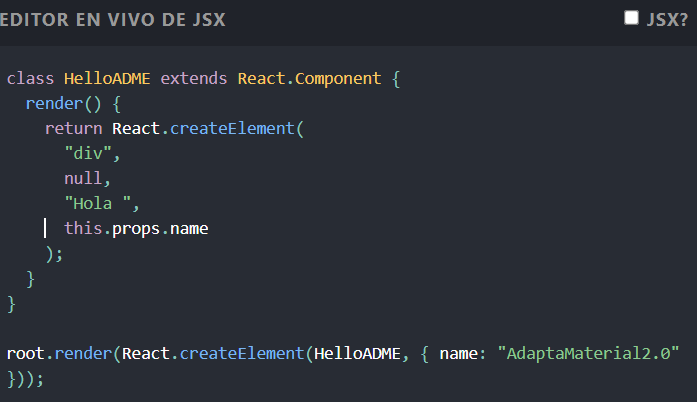
\includegraphics[width=0.6\textwidth]{Herraientas_Empleadas/ReactSinJSX.PNG}
      \caption{Componente sin JSX.}
      \label{SJSX}
    \end{subfigure}
    \caption{Componentes React}
    \label{fig:react}
  \end{figure}


\section{Material UI}\label{sec:MaterialUI}
Material UI\footnote{\url{https://mui.com/}} es una librería de componentes de React con estilos y funcionalidades predeterminadas. Estos componentes siguen un estilo de diseño llamado Material Design, que fue creado por Google y tiene una apariencia simple y profesional. Es bastante útil para implementar funcionalidades de una forma más rápida, ya que no hay que crear todos los componentes desde cero.

La librería permite añadir estilos personalizados al crear cada componente, sin necesidad de crear un fichero CSS propio, lo que permite hacer cambios con facilidad. También es bastante fácil realizar un diseño responsive gracias a las opciones que nos ofrece.

En nuestra aplicación, decidimos utilizar Material UI principalmente para implementar un componente que usamos en los modales de “Ejercicio de definiciones” y “Ejercicio de desarrollo”. Este componente es un selector que nos permite escoger el tipo de pauta que se usará en el ejercicio, por ejemplo, líneas normales, líneas de doble pauta, cuadrícula, etc. También permite seleccionar la separación entre las líneas y el tamaño de las celdas de la cuadrícula.

Podemos observar esta funcionalidad en la Figura \ref{selectorMaterialUI}.

\begin{figure}[ht!]
  \centering
  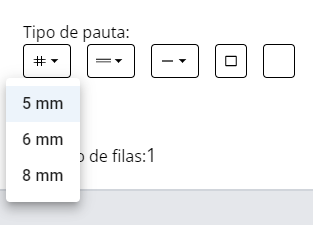
\includegraphics[width=0.6\textwidth]{Herraientas_Empleadas/SelectorMaterialUI.PNG}
  \caption{Selector de tipo de pauta}
  \label{selectorMaterialUI}
\end{figure}
